%!TEX root = ../main.tex

\chapter{Ottimizzazione con le Reti Neurali}
\label{cha:ottimizzazione_con_le_reti_neurali}
In questo capitolo saranno introdotti alcuni famosi problemi NP-difficili:\footnote{Un problema $P$ si dice \textbf{NP-difficile} se ogni problema $L \in NP$ è riducibile in tempo polinomiale a $P$. Un problema $P$ si dice \textbf{NP-completo} se $P \in NP$ ed è NP-difficile.} il problema del commesso viaggiatore (\emph{Traveling Salesman Problem}) e il problema della cricca massima (\emph{Maximum Clique Problem}). Dal momento che questi problemi non sono risolvibili in tempo polinomiale, sarà fornita una formulazione alternativa in modo tale da poter utilizzare tecniche di ottimizzazione continua per approssimare una soluzione.

\section{Problema del commesso viaggiatore}
\label{sec:problema_del_commesso_viaggiatore}

Il \textbf{problema del commesso viaggiatore} è il seguente: data una rete di città, trovare il percorso di lunghezza minima che un commesso viaggiatore deve seguire per visitare tutte le città una e una sola volta e poi tornare alla città di partenza.

\subsection{Formalizzazione del problema}

La rete di città può essere rappresentata mediante un grafo completo pesato $G = (V, E, w)$ dove $V$ è l'insieme delle città, $E$ l'insieme delle strade che le collegano e $w$ la funzione peso che assegna ad ogni arco la distanza tra i nodi corrispondenti. Il problema può dunque essere formalizzato come segue:
\begin{quote}
	\emph{Dato un grafo completo pesato $G=(V, E, w)$, trovare il ciclo di costo minimo (di lunghezza $|V|$) che tocchi tutti i nodi in $V$ una sola volta.}
\end{quote}
\vspace{-10pt}
\begin{figure}[h!]
	\centering
	\begin{tikzpicture}
        
		\node[circle,fill=blue!20] (A) at (0,2) {A};
		\node[circle,fill=blue!20] (B) at (-2,0) {B};
		\node[circle,fill=blue!20] (C) at (2,0) {C};
		\node[circle,fill=blue!20] (D) at (0, -2) {D};
        
		\foreach \from / \to in {B/A,B/D}
		\path (\from) edge[left] node {$w_{\from\to}$} (\to);
        
		\foreach \from / \to in {C/A,C/D}
		\path (\from) edge[right] node {$w_{\from\to}$} (\to);
             
		\path (A) edge[below left=0.1cm  of A] node {$w_{AD}$} (D);
		\path (B) edge[above right=0.1cm  of C] node {$w_{BC}$} (C);
             
	\end{tikzpicture}
	\caption{Grafo completo pesato.}\label{fig:graph}
\end{figure}

\subsection{Soluzione del TSP con le reti di Hopfield}
\label{sub:soluzione_del_tsp_con_le_reti_di_hopfield}

Per affrontare il problema utilizzando le reti di Hopfield è necessario trovare una \textbf{funzione di energia} adeguata, in modo tale che il minimo corrisponda alla soluzione del problema che si sta affrontando.

Per rappresentare il percorso si può usare una \textbf{matrice di permutazione}: dato il grafo in figura~\ref{fig:graph}, il percorso $B \rightarrow A \rightarrow C \rightarrow D$ può essere rappresentato con la matrice in tabella~\ref{tab:matperm}.

\begin{table}[h!]
	\centering
	\begin{tabularx}{8cm}{lXXXX}
		\toprule
		\backslashbox{Città}{Fermata} & 1 & 2 & 3 & 4 \\
		\midrule
		A & 0 & \textbf{1} & 0 & 0 \\
		B & \textbf{1} & 0 & 0 & 0 \\
		C & 0 & 0 & \textbf{1} & 0 \\
		D & 0 & 0 & 0 & \textbf{1} \\
		\bottomrule
	\end{tabularx}
	\caption{Matrice di permutazione del percorso BACD}
	\label{tab:matperm}
\end{table}

\noindent Per $n$ città sono quindi necessari $n^2$ neuroni nella rete di Hopfield, in cui ogni neurone identifica una città e una fermata. Introduciamo ora alcune notazioni:
\begin{itemize}
	\item $X$ indica una città;
	\item $i$ una fermata in cui è visitata una città;
	\item $V_{X,i}$ è l'output dell'unità $X, i$;
	\item $T_{Xi, Yj}$ sono i pesi delle connessioni;
	\item $V_{X,i} = 1$ se la città $X$ è visitata alla fermata $i$, $0$ altrimenti;
	\item $d_{X,Y}$ distanza tra la città $X$ e $Y$.
\end{itemize}
La funzione che rappresenta il costo totale del cammino è
\begin{align*}
	E_1  = \frac{D}{2} \sum_X \sum_{Y \neq X} \sum_i d_{X,Y} V_{X,i} (V_{Y, i-1} + V_{Y, i+1})
\end{align*}
dove $D$ è una costante positiva e gli indici sono intesi modulo $n$.

\begin{figure}[h!]
	\centering
    
	\subfigure{
	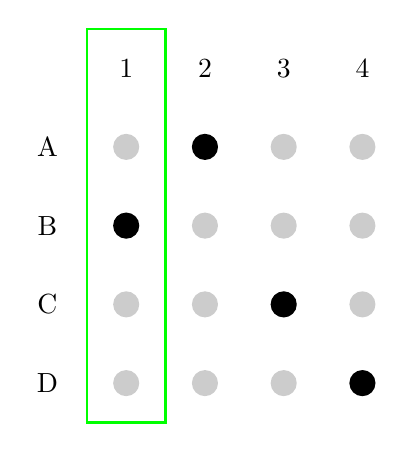
\begin{tikzpicture}
        
		\foreach \x / \y in {1/A,2/B,3/C,4/D} {
		\node (0-\x) at (0, -\x) {\y};
		\node (\x-0) at (\x, 0) {\x};
		}
        
		\foreach \x in {1,...,4} {
		\foreach \y in {1,...,4} 
		\node[circle, fill=black!20] (\x-\y) at (\x, -\y) {};
		}

		\foreach \x / \y in {1/2, 2/1, 3/3, 4/4} {
		\node[circle, fill=black] at (\x,-\y) {};
		}
        
		\draw[green, thick] (0.5,0.5) rectangle (1.5,-4.5);
        
	\end{tikzpicture}}
	\qquad
	\subfigure{
	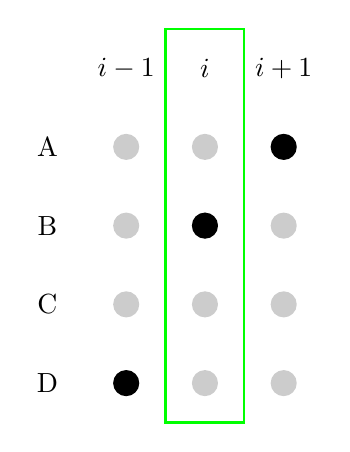
\begin{tikzpicture}
		\foreach \x / \y in {1/A,2/B,3/C,4/D}
		\node (0-\x) at (0, -\x) {\y};
        
		\foreach \x / \y in {1/$i-1$, 2/$i$, 3/$i+1$}
		\node (\x-0) at (\x, 0) {\y};
        
		\foreach \x in {1,...,3}
		\foreach \y in {1,...,4} 
		\node[circle, fill=black!20] at (\x, -\y) {}; 
                
		\foreach \x / \y in {4/1, 2/2, 1/3} {
		\node[circle, fill=black] at (\y,-\x) {};
        
		\draw[green, thick] (1.5,0.5) rectangle (2.5,-4.5);
		}
	\end{tikzpicture}}
	\caption{Interpretazione grafica di $E_1$}
\end{figure}

Per imporre i vincoli richiesti dal problema del commesso viaggiatore si introducono le seguenti funzioni di energia, che sono minimizzate quando i vincoli corrispondenti sono verificati.
\begin{itemize}
	\item \textbf{Vincolo sulle righe}. Ogni città deve essere visitata al più una sola volta:
	\begin{displaymath}
		E_2 = \frac{A}{2} \sum_X \sum_i \sum_{j \neq i} V_{X,i} V_{X,j}
	\end{displaymath}
	\item \textbf{Vincolo sulle colonne}. In una fermata si visita al più una città:
	\begin{displaymath}
		E_3 = \frac{B}{2} \sum_i \sum_X \sum_{Y \neq X} V_{X,i} V_{Y,i}
	\end{displaymath}
	\item \textbf{Vincolo sulle entrate}. Devono essere attraversate esattamente $n$ città:
	\begin{displaymath}
		E_4 = \frac{C}{2}\left(\sum_X \sum_i V_{X,i} - n \right)^2
	\end{displaymath}
\end{itemize}
Abbiamo quattro funzioni energia da minimizzare, tuttavia per poter utilizzare una rete di Hopfield è necessaria un'unica funzione: per questo motivo si esprime la funzione di costo totale come combinazione lineare delle funzioni energia $E_i$:
\begin{displaymath}
	E = E_1 + E_2 + E_3 + E_4
\end{displaymath}
dove il peso da attribuire a ciascun termine è determinato dalle costanti positive $A, B, C, D$. C'è un ultimo problema da risolvere, ovvero la funzione energia dovrà essere della forma tipica di una rete di Hopfield:
\begin{displaymath}
	E = - \frac{1}{2} \sum_{X, Y} \sum_{i, j} T_{Xi, Yj} V_{X, i} V_{Y, j} - \sum_{X, i} I_{X, i} V_{X, i}
\end{displaymath}
Per farlo, si introduce il termine
\begin{displaymath}
	\delta_{i,j} = \begin{cases}
		1 & \text{se } i = j \\
		0 & \text{altrimenti}
	\end{cases}
\end{displaymath}
e si riscrivono le funzioni $E_i$ come segue:
\begin{align*}
	E_1 &= \frac{D}{2} \sum_X \sum_{Y \neq X} \sum_i d_{X,Y} V_{X,i} (V_{Y, i+1} + V_{Y, i-1}) \\
	&=  \frac{D}{2} \sum_{X,Y} \sum_{i,j} d_{X,Y} V_{X,i} V_{Y,j} (\delta_{j, i-1} + \delta_{j, i+1})
\end{align*}

\begin{align*}
	E_2 &= \frac{A}{2} \sum_X \sum_i \sum_{j \neq i} V_{X,i} V_{X,j} \\
	&= \frac{A}{2} \sum_{X,Y} \sum_{i,j} V_{X,i} V_{Y,j} \delta_{X,Y} (1 - \delta_{i,j})
\end{align*}

\begin{align*}
	E_3 &= \frac{B}{2} \sum_i \sum_X \sum_{Y \neq X} V_{X,i} V_{Y,i} \\
	&= \frac{B}{2} \sum_{X,Y} \sum_{i,j} V_{X,i} V_{Y,j} \delta_{i,j} (1 - \delta_{X,Y})
\end{align*}

\begin{align*}
	E_4 &= \frac{C}{2}\left(\sum_X \sum_i V_{X,i} - n \right)^2 \\
	&= \frac{C}{2} \left(\left(\sum_X \sum_i V_{X,i}\right)^2 - 2n \sum_X \sum_i V_{X,i} + n^2 \right)
\end{align*}
dove
\begin{align*}
	\left(\sum_X \sum_i V_{X,i}\right)^2 &= \left(\sum_X \sum_i V_{X,i}\right) \left(\sum_X \sum_i V_{X,i} \right) \\
	&= \sum_{X,Y} \sum_{i,j} V_{X,i} V_{Y,j}
\end{align*}

\newpage

\noindent In $E_4$ il termine costante $n^2$ si può tralasciare, in quanto influenza solamente il valore della funzione $E_4$ in corrispondenza del minimo, ma non la sua posizione. Mettendo il tutto assieme si ottiene la \textbf{funzione di energia totale}
\begin{align*}
	E &= \frac{A}{2} \sum_{X,Y} \sum_{i,j} V_{X,i} V_{Y,j} \delta_{X,Y} (1 - \delta_{i,j}) \\
	&+ \frac{B}{2} \sum_{X,Y} \sum_{i,j} V_{X,i} V_{Y,j} \delta_{i,j} (1 - \delta_{X,Y}) \\
	&+ \frac{C}{2} \left(\sum_{X,Y} \sum_{i,j} V_{X,i} V_{Y,j} - 2n \sum_{X,i} V_{X,i} \right) \\
	&+ \frac{D}{2} \sum_{X,Y} \sum_{i,j} d_{X,Y} V_{X,i} V_{Y,j} (\delta_{j, i-1} + \delta_{j, i+1}) \\
	&= - \frac{1}{2} \sum_{X, Y} \sum_{i, j} T_{Xi, Yj} V_{X, i} V_{Y, j} - \sum_{X, i} I_{X, i} V_{X, i}
\end{align*}
dove $T_{Xi, Yj}$ sono dati da
\begin{align*}
	-T_{Xi, Yj} &= A \delta_{XY} (1 - \delta_{ij}) \tag{Peso inibitorio in ogni riga}\\
	& +B \delta_{ij} (1 - \delta_{XY}) \tag{Peso inibitorio in ogni colonna} \\
	& +C  \qquad \tag{Inibizione globale}\\
	& +D d_{XY} (\delta_{j,i-1} + \delta_{j, i+1}) \tag{Costo del cammino minimo}
\end{align*}
e il vettore di corrente esterna $\vec{I}$ ha come $Xi$-esima componente
\begin{align*}
	I_{X, i} = nC\tag{Corrente esterna eccitatoria}
\end{align*}

\subsection{Un'altra formulazione}
\label{sub:un_altra_formulazione}

Determinare i parametri $A, B, C, D$ è particolarmente difficile. Un altro modo per esprimere i vincoli del TSP, che richiede di determinare un parametro in meno è il seguente:
\begin{align*}
	E_2 = \frac{A}{2} \sum_X \left(\sum_i V_{X, i} - 1 \right) ^ 2 \tag{Vincolo sulle righe} \\
	E_3 = \frac{B}{2} \sum_i \left(\sum_X V_{X, i} - 1 \right) ^ 2 \tag{Vincolo sulle colonne} \\
\end{align*}
La funzione energia diventa:
\begin{align*}
	E = \frac{D}{2} \sum_{X} \sum_{Y \neq X} \sum_i d_{X,Y} V_{X,i}(V_{Y, i + 1} + V_{Y, i - 1}) + E_2 + E_3
\end{align*}

\subsection{Problema delle N regine}
\label{sub:problema_delle_n_regine}

Una famosa variante del TSP è il \textbf{problema delle N regine}: data una scacchiera $N \times N$ e $N$ regine, si vogliono posizionare questi pezzi in modo tale che nessuno di essi possa attaccarne un altro.

Si può costruire una rete di Hopfield $N \times N$ in cui il neurone $(i,j)$ è attivo se e solo se una regina occupa la posizione $(i,j)$, con i seguenti vincoli:
\begin{itemize}
	\item solo una regina in ciascuna riga;
	\item solo una regina in ciascuna colonna;
	\item solo una regina in ciascuna diagonale;
	\item solo $N$ regine sulla scacchiera.
\end{itemize}
Il problema è analogo al TSP con l'aggiunta del vincolo sulle diagonali. La matrice dei pesi è la seguente:
\begin{align*}
	- T_{ij,kl} &= A \delta_{ik} (1 - \delta_{jl}) \tag{Peso inibitorio in ogni riga}\\
	& + B \delta_{jl} (1 - \delta_{ik}) \tag{Peso inibitorio in ogni colonna} \\
	& + C \tag{Inibizione globale}\\
	& + D (\delta_{i+j,k-l} + \delta_{i-j, k-l})(1 - \delta_{ik}) \tag{Peso inibitorio sulle diagonale}
\end{align*}

\subsection{Conclusioni}

L'ottimizzazione tramite le reti di Hopfield presenta alcuni svantaggi:
\begin{enumerate}
	\item sono necessari $n^2$ neuroni;
	\item il numero di connessioni è $\mathcal{O}(n^4)$;
	\item i parametri $A, B, C, D$ sono difficili da determinare;
	\item i risultati ottenuti sono raramente soluzioni ammisibili, ovvero matrici binarie con i vincoli rispettati;
	\item è difficile evitare i minimi locali della funzione di energia.
\end{enumerate}

\newpage

\section{Problema della cricca massima}
\label{sec:problema_della_cricca_massima}

Sia $G=(V,E)$ un grafo non orientato: si definisce \textbf{cricca} (o \emph{clique}) un sottoinsieme $C \subseteq V$ di vertici mutuamente adiacenti, ovvero tali per cui $\forall i,j \in C$, se $i \neq j$, allora $(i,j) \in E$.
\begin{mydef}[Clique massimale]
	Si definisce \defterm{clique massimale} di $G$ una clique di $G$ che non è contenuta in nessun'altra clique di $G$.\footnote{Se $C$ è una clique massimale, allora ogni nodo $j \notin C$ è connesso a meno di $|C|$ nodi della clique. Se è connesso a meno di $|C| - 1$ nodi, la clique è massimale \textbf{stretta}.}
\end{mydef}
\begin{mydef}[Clique massima]
	Si definisce \defterm{clique massima} di $G$ una clique massimale di G di cardinalità massima.
\end{mydef}
\noindent Il problema consiste nel trovare una cricca massima (MCP).

\begin{figure}[h!]
	\centering
	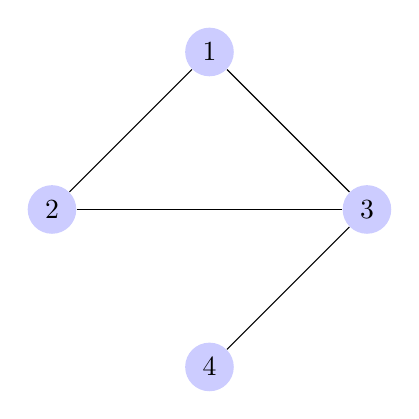
\begin{tikzpicture}
		\node[circle,fill=blue!20] (1) at (0,2) {1};
		\node[circle,fill=blue!20] (2) at (-2,0) {2};
		\node[circle,fill=blue!20] (3) at (2,0) {3};
		\node[circle,fill=blue!20] (4) at (0, -2) {4};
    
		\foreach \from / \to in {1/2,2/3,1/3,3/4}
		\path (\from) edge (\to);
	\end{tikzpicture}
	\caption[Esempi di clique.]{$C_1 = \{1, 2, 3\}$ è massima e massimale, $C_2 = \{3, 4\}$ è massimale, \\ $C_3 = \{1, 2\}$ non è massimale ($C_3 \subseteq C_1$).}
\end{figure}

\noindent Trovare una clique massimale è un problema facile, mentre trovare quella massima è NP-completo, così come trovare la dimensione di tale clique. 

Prima di dare una formulazione continua del problema della cricca massima, sono necessarie alcune definizioni:
\begin{itemize}
	\item Se $C \subseteq V$, $\vec{x}^C$ indica il \textbf{vettore caratteristico} di $C$:
	\begin{displaymath}
		x^C_i = \begin{cases}
			\displaystyle\frac{1}{|C|} &\text{se }i \in C\\
			0 &\text {altrimenti}
		\end{cases}
	\end{displaymath}
	\item $\Delta$ è il \textbf{simplesso standard} in $\mathbb{R}^n$:
	\begin{displaymath}
		\Delta = \left\{\vec{x} \in \mathbb{R}^n : \sum_{i=1}^n x_i = 1 \text{ e } x_i \geq 0, \forall i \right\}
	\end{displaymath}\newpage
	\item $\mat{A} = (a_{ij})$ è la matrice di adiacenza binaria di $G$.
\end{itemize}

\begin{figure}[t]
	\centering
	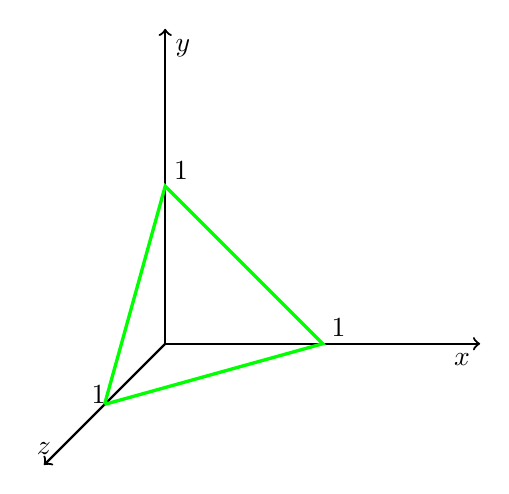
\begin{tikzpicture}[scale=2]

		%draw the main coordinate system axes
		\draw[thick,->] (0,0,0) -- (2,0,0) node[anchor=north east]{$x$};
		\draw[thick,->] (0,0,0) -- (0,2,0) node[anchor=north west]{$y$};
		\draw[thick,->] (0,0,0) -- (0,0,2) node[anchor=south]{$z$};
        
		\draw[thick, color=green, very thick] plot coordinates{(0,0,1) (0,1,0) (1,0,0) (0,0,1)};
        
		\node at (1.1,0.1,0) {1};
		\node at (0.1,1.1,0) {1};
		\node at (0,0.1,1.1) {1};
        
	\end{tikzpicture}
	\caption{Simplesso standard in $\mathbb{R}^3$.}
\end{figure}

\noindent Si consideri la seguente funzione quadratica detta \textbf{Lagrangiano del grafo}:
\begin{displaymath}
	f_G(\vec{x}) = \vec{x}^T \mat{A} \vec{x} = \sum_{i=1}^n \sum_{j=1}^n a_{ij} x_i x_j
\end{displaymath}
L'approccio tipico per risolvere il problema della cricca massima è quello di costruire un sistema dinamico che converga ai massimi di $f_G$ in $\Delta$: questi punti corrisponderanno alle soluzioni nello spazio discreto del problema originale. A tale scopo si introduce il teorema di Motzkin-Straus.
\begin{thm}[T. S. Motzkin \& E. G. Straus, 1965]
	Sia $\vec{x}^*$ un massimo globale di $f_G$ in $\Delta$, allora la cardinalità della clique massima di $G$ è legata a $f_G$ dalla seguente formula:
	\begin{displaymath}
		\omega(G) = \frac{1}{1 - f_G(\vec{x}^*)}
	\end{displaymath}
	Inoltre un sottoinsieme di vertici $C$ è una clique massima se e solo se il suo vettore caratteristico $\vec{x}^C \in \Delta$ è un massimo globale per $f_G$ in $\Delta$.
\end{thm} 
\noindent Purtroppo non tutti i massimizzatori di $f_G$ sono nella forma di vettori caratteristici, pertanto possono essere usati solo per ottenere la cardinalità della cricca massima, ma non i vertici che la compongono: questi massimizzatori sono detti \textbf{soluzioni spurie}.

Ad esempio, il grafo in figura \ref{fig:grafoesempio} contiene due clique massime:
\begin{align*}
	C_1 &= \{1,2\} & \vec{x}^{C_1} &= (1 / 2, 1 / 2, 0) \\
	C_2 &= \{1,3\} & \vec{x}^{C_2} &= (1 / 2, 0, 1 / 2)
\end{align*}

\begin{figure}[h!]
	\centering
	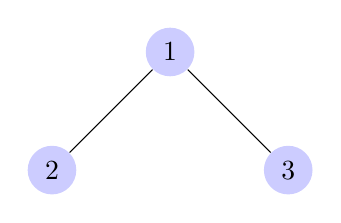
\begin{tikzpicture}
		\node[circle,fill=blue!20] (1) at (0,1.5) {1};
		\node[circle,fill=blue!20] (2) at (-1.5,0) {2};
		\node[circle,fill=blue!20] (3) at (1.5,0) {3};
        
		\draw (1) -- (2);
		\draw (1) -- (3);
        
	\end{tikzpicture}
	\caption{Grafo di esempio.}
	\label{fig:grafoesempio}
\end{figure}

\noindent Tuttavia, come si può vedere dal seguente grafico, sono massimi globali tutti i punti interni al segmento $\vec{x}^{C_1}\vec{x}^{C_2}$ ovvero i punti $(1/2, \alpha / 2, (1 - \alpha) / 2)$ con $\alpha \in (0,1)$: tuttavia, poiché non sono nella forma di vettori caratteristici, non possono essere usati per estrarre informazioni sui componenti delle clique massime.
\begin{figure}[h!]
	\centering
	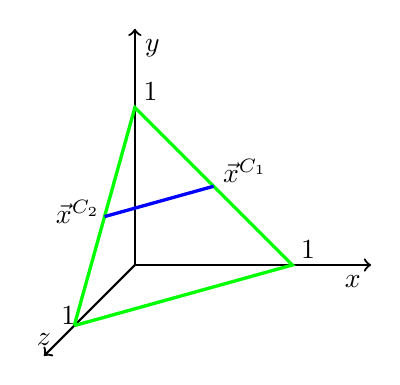
\begin{tikzpicture}[scale=2]
		%draw the main coordinate system axes
		\draw[thick,->] (0,0,0) -- (1.5,0,0) node[anchor=north east]{$x$};
		\draw[thick,->] (0,0,0) -- (0,1.5,0) node[anchor=north west]{$y$};
		\draw[thick,->] (0,0,0) -- (0,0,1.5) node[anchor=south]{$z$};
        
		\draw[thick, color=green, very thick] plot coordinates{(0,0,1) (0,1,0) (1,0,0) (0,0,1)};
		\draw[color=blue, very thick] (.5, .5, 0) -- (0,.5,.5);
        
		\node at (.7,.6,0) {$\vec{x}^{C_1}$};
		\node at (-.15,.55,.55) {$\vec{x}^{C_2}$};
        
		\node at (1.1,0.1,0) {1};
		\node at (0.1,1.1,0) {1};
		\node at (0,0.1,1.1) {1};
        
	\end{tikzpicture}
	\caption{Soluzioni spurie in MCP}
\end{figure}

\noindent Il problema delle soluzioni spurie è stato risolto da Bomze proponendo una versione regolarizzata di $f_G(\vec{x})$:
\begin{displaymath}
	\hat{f}_G(\vec{x}) = \vec{x}^T \left(\mat{A} + \frac{1}{2} \mat{I}_{|V|} \right) \vec{x} 
\end{displaymath}

\begin{thm}[I. M. Bomze, 1995]
	Sia $C \subseteq V$ e sia $\vec{x}^C$ il suo vettore caratteristico, allora:
	\begin{itemize}
		\item $C$ è una clique massima di $G$ se e solo se $\vec{x}^C$ è un massimo globale di $\hat{f}_G$ in $\Delta$;
		\item $C$ è una clique massimale di $G$ se e solo se $\vec{x}^C$ è un massimo locale di $\hat{f}_G$ in $\Delta$;
		\item ogni massimo locale è un vettore caratteristico ed è locale stretto. 
	\end{itemize}
\end{thm}
